\documentclass{article}





\usepackage[utf8]{inputenc} % allow utf-8 input
\usepackage[T1]{fontenc}    % use 8-bit T1 fonts
\usepackage{hyperref}       % hyperlinks
\usepackage{url}            % simple URL typesetting
\usepackage{booktabs}       % professional-quality tables
\usepackage{amsfonts}       % blackboard math symbols
\usepackage{nicefrac}       % compact symbols for 1/2, etc.
\usepackage{microtype}      % microtypography
\usepackage{xcolor}         % colors
\usepackage{graphicx}       % addtional package for show figures


\begin{document}


\maketitle

%%%%%%%Part 2 Annotation Quality Start%%%%%%%%%

\section{Annotation Quality}

\subsubsection{(a) Precision of temporal annotations}
We assessed the precision of temporal annotations by analyzing the duration of overlapping annotations (Table~\ref{tab:dur}). The standard deviation was approximately 10 seconds, and the inter-quartile range exceeded 20 seconds, suggesting significant variability.
However, annotators agreed on the number of distinct sound events in 94.7\% of cases, indicating consistency in event identification despite differences in duration. 

\begin{table}[h]
    \caption{Summary Statistics of Duration of Overlapping Annotations.}
    \label{tab:dur}
    \centering
    \begin{tabular}{lcl}
        \toprule
        Statistic & Duration (in seconds) \\ \midrule
        Mean            & 10.694948 \\
        Std             & 10.100707 \\
        Min             & 0.052521 \\
        25\%            & 1.343494 \\
        50\%            & 5.799818 \\
        75\%            & 20.679048 \\ 
        Max             & 30.044718 \\ \bottomrule
    \end{tabular}
\end{table}


\subsubsection{(b) Similarity of textual annotations}
We measured textual similarity in overlapping regions using annotation length and cosine similarity. Text length varied significantly, with a standard deviation of 4.33 words.
Cosine similarity analysis (Table~\ref{tab:cos}) revealed low agreement among annotators, with a mean of 0.06 and an inter-quartile range from -0.03 to 0.14. This suggests that descriptions often differed substantially, and in some cases, even opposed each other.  

\begin{table}[h]
    \caption{Summary Statistics of Cosine Similarity of Overlapping Annotations.}
    \label{tab:cos}
    \centering
    \begin{tabular}{lcl}
        \toprule
        Statistic & Cosine Similarity \\ \midrule
        Mean            & 0.063015 \\
        Std             & 0.144213 \\
        Min             & -0.357656 \\
        25\%            & -0.032708 \\
        50\%            & 0.049751 \\
        75\%            & 0.140056 \\ 
        Max             & 0.848671 \\ \bottomrule
    \end{tabular}
\end{table}

\subsubsection{(c) Frequency of annotations and sound events}
Each sound file contained an average of 3.99 annotations and 3.72 distinct sound events, with a minimum of 1, The minimum is reasonable considering that some files may contain a single continuous sound.

\subsubsection{(d) Detail of annotations}
The level of detail in individual annotations varied significantly. The distribution of annotation lengths displayed in Figure~\ref{fig:len} is positively skewed, suggesting that most descriptions were brief, with a median of 7 words.

\begin{figure}[h]
    \centering
    %Elbow+Silhouette plot
    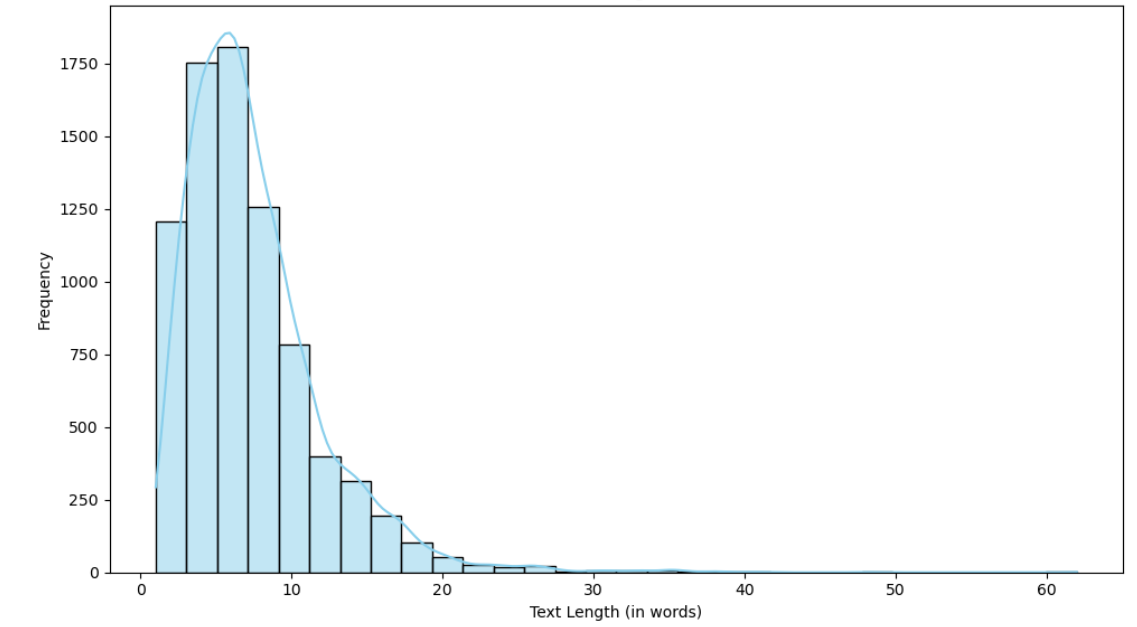
\includegraphics[width=.55\linewidth]{distribution_of_text_lengths.PNG}
    \caption{Distribution of Text Lengths in Annotations.}
    \label{fig:len}
\end{figure}

\subsubsection{(d) Inconsistencies and outliers}
No technical errors were found (e.g., offsets preceding onsets or zero-duration annotations) and these checks could be implemented automatically.
Regarding the content ,annotations with zero or very short lengths (<2 words) may be considered inadequate. However, using statistical outlier detection (e.g., IQR) may be overly limiting and could flag valid annotations.


%%%%%%%Part 2 Annotation Quality Finish%%%%%%%%%


\end{document}